
% -----------------------------------------------
% Domain & Problem
% -----------------------------------------------

In times of battling the climate crisis,
organizations are challenged with optimizing their processes
in order to drive sustainable development.
% adhering to stricter regulations regarding their carbon footprints.
The implementation of emissions trading hereby requires reporting of Greenhouse Gas (GHG) emissions, referred to as Carbon Accounting (CA).

Employing Object-Centric Process Mining (OCPM) offers a holistic view of the as-is process utilizing event data associated with objects of different types~\cite{vanderAalst19object}.
OCPM is enabled by extracting such event data from information systems that support the process.
However, these information systems typically do not contain data on sustainability indicators such as carbon footprints~\cite{Brehm22process}.
Assuming such data were available,
OCPM could provide multi-perspective sustainability insights,
such as identifying emission-driving activities or object types within the process~\cite{Brehm22process,Graves23rethink}.
Moreover, it enables calculating object carbon footprints. This is closely related to the concept of Life-Cycle Assessment (LCA)~\cite{Graves23rethink},
that involves identifying environmental impacts associated with a product over the course of its lifecycle~\cite{Ortmeier21framework}.

The recent OCEL~2.0 standard provides an interchangeable format for Object-Centric Event Logs (OCELs)~\cite{OCEL2}. However, there are currently no approaches addressing the aforementioned tasks based on these data.
In general, applying OCPM for sustainability assessment has been encouraged,
but contributions are mostly limited to theoretical frameworks~\cite{Graves23rethink,Ortmeier21framework}.

% -----------------------------------------------
% Method
% -----------------------------------------------
In this work,
we propose a method for
1)\ deriving emissions from an OCEL based on hand-selected emission factors,
2)\ aggregating emissions to total event emissions,
and 3)\ allocating emissions from events to objects.
To make this practically applicable, the OCEAn web application
(short for \textbf{O}bject-\textbf{C}entric \textbf{E}mission \textbf{An}alysis)
is implemented,
allowing for the application of OCPM in CA and for exporting resulting data to form a basis for further research.

Hereby, emission estimation is achieved by allowing the user to define and apply emission rules, combining hand-selected emission factors with event data including attribute values from an OCEL.
The resulting carbon footprints are then integrated into the log, allowing for a file export for further use.
%
The second and third contribution demonstrate OCPM's capabilities of offering multi-dimensional views to the process -- and in this case, to the emissions associated with its events.
After selecting the perspective, i.e., an object type, the event emissions are allocated to the objects of that type, resulting in object carbon footprints, thus addressing LCA.
%
Object allocation involves the use of an allocation rule that selects the objects related most directly to each event. We propose three allocation rules of different complexities.
A special treatment of process resources like machines, employees or vehicles is advised in multiple OCPM approaches~\cite{Graves23rethink,Fahland22process}.
Resources are found to have longer lifecycles and more interacting objects than objects of other types, referred to as Handling Units (HUs).
Object allocation considers this distinction, optionally disregarding interactions with resource objects.

% -----------------------------------------------
% Evaluation & Results
% -----------------------------------------------
An evaluation is conducted in order to compare the allocation rules proposed
w.r.t. their resulting object emission distributions using suitable measures.
Furthermore, runtime of the most complex allocation rule is recorded, examining potential speedups while considering implications on result preservation.
Based on these findings, the OCEAn application is equipped with functionality to execute object allocation employing the best-performing rule.
% Together with the OCEL standard~\cite{OCEL2}, a set of example event logs has been published.
% Most of them contain artificial data as a result of simulation~\cite{orderManagement,containerLogistics,p2p}.
% Following the implementation of the OCEAn app, the object allocation framework is evaluated using these OCELs. To this end, all combinations of parameters and allocation rules are executed.
% Allocation results are then described by suitable statistics allowing for comparison of the different allocation rules depending on the input data structures.

% ---------------------------------------------------------------------
% ---------------------------------------------------------------------
\section{Motivation}
\label{sec:intro-motiv}
% ---------------------------------------------------------------------
% ---------------------------------------------------------------------

\begin{figure}[t]
  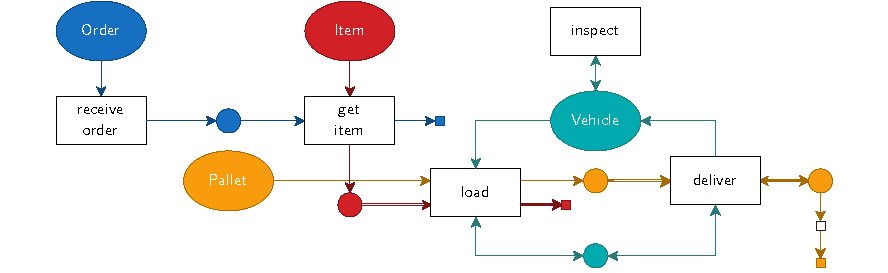
\includegraphics[width=\textwidth]{figures/concept/rex-logistics-ocpn.pdf}
  \caption{Process model of an example logistics process. Orders consist of multiple items, that are loaded onto pallets and into vehicles. A vehicle delivers the pallets to customers and needs to undergo regular inspection.}
  \label{fig:rex-ocpn}
\end{figure}

In the following, the potential of OCEL~2.0 data for the aforementioned emission analysis tasks is illustrated.
To this end, consider an example process of an imaginary logistics provider.
The company operates \otype{vehicles} for delivering large goods, leading to carbon emissions.
The process starts with receiving an \otype{order} that consists of one or more \otype{items}.
Items are then loaded onto vehicles using \otype{pallets}.
\otype{Pallets} can contain multiple items of the same order. Pallets of multiple orders may be delivered together, unloading one after the other from the vehicle.
Next to the \activity{deliver} activity, the vehicles need to undergo regular inspection, involving additional journeys.
A model of this process is shown in \autoref{fig:rex-ocpn}.

We assume an OCEL of the given process is extracted from an information system,
containing records of events and objects together with attributes such as journey distances and average fuel consumption.
However, emission data are not captured in the information system.
Therefore, they are also missing in the OCEL.
Still, the company wants to report the emissions caused by the process. More precisely, the goal is to
\begin{itemize}
	\item estimate event-level emissions in a bottom-up fashion leveraging the event data,
	\item detect emission drivers based on these emission data such as specific activities,
	\item allocate all process emissions to objects of a given type, e.g., orders or items.
\end{itemize}

For simplicity, we assume that only the activities \activity{deliver} and \activity{inspect} cause emissions due to driving the vehicle.
In order to estimate vehicle emissions, the fuel consumption of each journey is approximated by multiplying an average fuel consumption with the journey distance.
Finally, an emission factor database is searched to obtain a \COtwo{} equivalent.
Assuming the vehicle consumes \qty{12.5}{\liter\per\Ckm} and travels \qty{20}{\km}, applying an appropriate emission factor
\footnote{
	``Emission intensity of diesel (without biofuel content) per liter used in vehicle''
  -- source: GEMIS
  (\url{https://www.climatiq.io/data/emission-factor/d56128ea-76e5-4a31-a6fe-b5e1ed855e52})
}
yields the event emission estimate
\begin{align*}
	\qty{3.055}{\kgcotwoe\per\liter} \cdot \qty{12.5}{\liter\per\Ckm} \cdot \qty{20}{\km} &= \qty{7.6375}{\kgcotwoe}.
\end{align*}
Performing this computation for each event in the OCEL offers process insights in the next step:
For example, aggregating all event emissions by the event's activity, the overall emission share of inspection journeys can be computed
\footnote{In this example, just considering distances allows for the same comparison.
Emission estimation only adds value as soon as different activities employ different emission factors.}.

Moreover, the company wants to assess the emissions caused by each order and each item.
This adds two additional perspectives in which overall process emissions are fully distributed among these target objects.
To this end, all emissions along an object's lifecycle within the process are added to obtain a carbon footprint.
This way, LCA is performed on the selected objects, with the system boundaries here defined by the scope of the process data, i.e., within the logistics company.
Upstream emissions from producing an item are not included, neither are emissions caused by the use phase or disposal of the product.
After computing carbon footprints on either \otype{order} or \otype{item} level,
more process insights are gained.
For example, the impact of merging multiple deliveries can be assessed.

\begin{figure}[t]
	\centering
	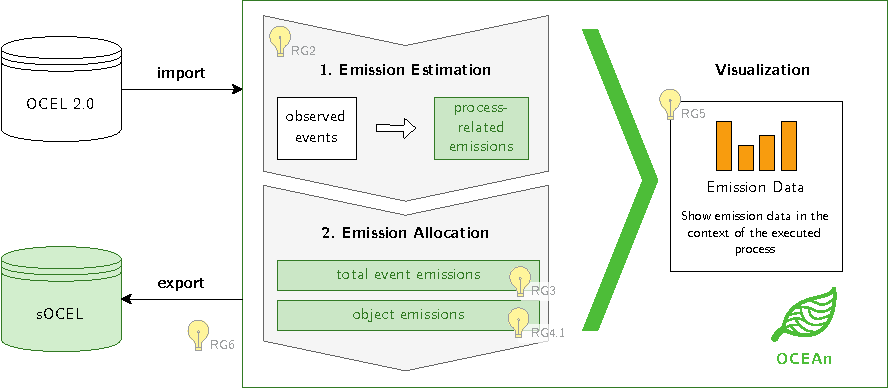
\includegraphics[width=.9\textwidth]{figures/concept/method-overview-1-intro.pdf}
	% \missingfigure[figwidth=.75\textwidth,figheight=6cm]{\Large Method intro figure}
	\caption{Contributions of the OCEAn application. First, event emissions are estimated by defining emission rules for different activities. Second, two perspectives on these emissions are offered in order to identify impacts of different activities or objects.}
	\label{fig:intro-method-overview}
\end{figure}

The OCEAn application enables solving all three previously mentioned problems.
\autoref{fig:intro-method-overview} depicts these use cases and the methods proposed, divided in two phases:
First, emission estimation allows bottom-up event emission computation using an emission factor selected by the user.
Second, emission allocation offers different perspectives on emission data, including the event perspective, and the object perspective.

Object allocation involves identifying relations between events and objects.
OCELs contain such relations (objects participating in events), however, these data are not sufficient:
In the above example, neither \otype{orders} nor \otype{items} participate in a delivery.
Therefore, we propose an \textit{object allocation framework} employing different allocation rules in order to find more links between events and the objects in question.

Apart from possible applications like in the above example, OCEAn aims at providing the research community with emission-annotated datasets and thus enabling further research.
To this end, it is built to work with event data in the OCEL~2.0 file format~\cite{OCEL2},
and allows integrating the computed emission values into that format
in order to obtain a sustainability-enriched OCEL (sOCEL).

%
% For this, it is assumed that the reporting scope is identical to those activities captured in the event log and our process model.

% ---------------------------------------------------------------------
% ---------------------------------------------------------------------
\section{Research Questions and Goals}
\label{sec:intro-rqs-rgs}
% ---------------------------------------------------------------------
% ---------------------------------------------------------------------

To structure the work, the problem statement from the previous section is divided in seven research questions (RQs).

\begin{enumerate}[label={RQ\arabic*},ref={RQ\arabic*},leftmargin=1.25cm,labelwidth=1cm,align=left]
	%
	\item How are techniques from PM used to carry out carbon emission analysis? How does OCPM improve applicability?
	\label{rq:1-rw}
	%
	\item How can process-related emissions be estimated using the data available in an OCEL?
	\label{rq:2-est}
	%
	\item How can the emissions recorded in the event log be aggregated and distributed to gain sustainability insights w.r.t. the different events and activities?
	\label{rq:3-events}
	%
	\item[RQ4a] How can the emissions recorded in the event log be aggregated and distributed to gain sustainability insights w.r.t. a specific subset of objects as required by LCA?
	\label{rq:4a-obj-lca}
	%
	\item[RQ4b] What characteristics of the event log impact the results of different allocation techniques in terms of performance and emission distribution?
	\label{rq:4b-obj-eva}
	%
	\setcounter{enumi}{4}
	\item What process-related sustainability insights can be directly gained by considering emission data in the context of an OCEL?
	\label{rq:5-insights}
	%
	\item How can the integration of emission data serve as a first step for a practical application of PM for sustainability?
	\label{rq:6-eva}
	%
\end{enumerate}


% % ---------------------------------------------------------------------
% % ---------------------------------------------------------------------
% \section{Research Goals}
% \label{sec:intro-rgs}
% % ---------------------------------------------------------------------
% % ---------------------------------------------------------------------

In the following, research goals are defined in order to answer the previously defined research questions.
% Before addressing the contributions of our web application, the first research goal is about getting familiar with related work.

\begin{enumerate}[label={RG\arabic*},ref={RG\arabic*},leftmargin=1.25cm,labelwidth=1cm,align=left]
	%
	\item\label{rg:1-rw}
	Investigation of previous works employing process mining for carbon emission analysis, as well as advances in OCPM influencing this.
	%
	\item\label{rg:2-est}
	Development and implementation of a method that uses the expressiveness of an OCEL to estimate emissions caused by behavior observed in the event log.
	%
	\item\label{rg:3-events}
	Development and implementation of a method to support the aggregation and distribution of the process emissions to events and activities.
	%
	\item[RG4a]\label{rg:4a-obj-framework}
	Development and implementation of methods for the allocation of process-related emissions to a subset of objects.
	%
	\item[RG4b]\label{rg:4b-obj-eva}
	Identification of OCEL characteristics that impact the results of allocation techniques in terms of performance and emission distribution.
	%
	\setcounter{enumi}{4}
	\item\label{rg:5-viz} Visualization of emission data derived from an OCEL to support the identification of basic process-related sustainability insights.
	%
	\item\label{rg:6-ocean-export} Provide a web application supporting the estimation and integration of process-related emissions as well as the export of an OCEL enhanced by these data.
	%
\end{enumerate}

The remainder of this thesis is structured as follows:
\autoref{chap:rw} addresses related work in order to pursue \RGone.
Following this, mathematical backgrounds and OCELs are introduced.
% in \autoref{chap:prelim}.
\autoref{chap:method} establishes the methods used in both phases,
including emission estimation (\RGtwo){} and emission allocation (\RGthree, \RGfourA).
After evaluating the allocation framework in \autoref{chap:eva} to address \RGfourB,
results and possible extensions are discussed in \autoref{chap:discussion}.
\autoref{chap:impl} gives implementation details of the OCEAn app and shows a potential user journey, summarizing the contributions to \RGfive{} and \RGsix.
The thesis is concluded with \autoref{chap:conclusion}.
